\begin{figure}
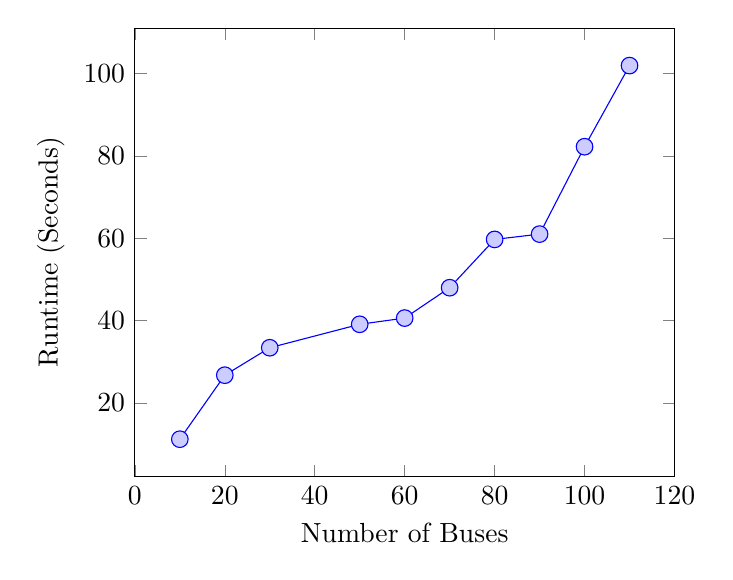
\begin{tikzpicture}
\begin{axis}[xlabel=Number of Buses, ylabel=Runtime (Seconds), legend pos=north west]
	\addplot[blue] coordinates {
		(10, 11.18)   
	  (20, 26.74)  
		(30, 33.41)  
		(50, 39.11)  
		(60, 40.62)  
		(70, 48.00)  
		(80, 59.74)  
		(90, 61.03)
		(100, 82.27)
		(110, 101.99)}; 
\addplot[blue!20, draw=blue, only marks, mark size=3pt] coordinates {
		(10, 11.18)   
	  (20, 26.74)  
		(30, 33.41)  
		(50, 39.11)  
		(60, 40.62)  
		(70, 48.00)  
		(80, 59.74)  
		(90, 61.03)
		(100, 82.27)
		(110, 101.99)};
\end{axis}
\end{tikzpicture}
\caption{Runtime comparison for different numbers of buses}
\label{fig:results:scalabilityRuntimes}
\end{figure}
